%Author: Jackson Perry
\section{The Dataset}

%The data arrived from DraftKings in a number of files over the course of four months. A large chunk of data came at the beginning of the project in September, followed by a supplementary portion in January 2019. 
The data consists of two main categories: what we call \textbf{Header Data} and \textbf{Time Series Data}. In this section, we will explore both categories, describe the magnitude and makeup of the datasets and explore some characteristics of the set.

\subsection{Header Data}

The Header Data in our set consists of all the label information for each of the hundreds of thousands of DraftKings contests over the last three years. A typical contest might be an NFL contest where users pay \$5 to enter, select a team of players in that week's games, then earn points as those players compete. If the user scores the most points of everyone entered into that specific contest, they can win the top prize or any number of secondary prizes. For a given contest, we were provided the following 21 header columns of data, found in Table \ref{tab:headercols}. 

\begin{table}
\centering
\begin{tabular}{|p{5cm}|p{1.6cm}|p{9.5cm}|}
\hline
 \textbf{Feature Name} & \textbf{Data Type} & \textbf{Description}  \\ 
    \hline
    ContestId & Integer & a unique 7- or 8-digit number identifying each contest \\
    \hline
    DraftGroupId & Integer & number identifying a unique SportName, VariantName and ContestStartDatetimeEST combination\\ %which group of players is able to be drafted in that contest 
    \hline
    SportName & String & a three or four character string describing the sport of the contest\\
    \hline
    VariantName & String & a string description of the type of contest \\
    \hline
    GameSet & String & a string description of the time of day that the contest runs \\
    \hline
    ContestName & String & the string describing the contests that users see \\
    \hline
    ContestStartDatetimeEST & Datetime Object & when the contest opens to be entered by users \\
    \hline
    ContestEndDatetimeEST & Datetime Object & when the contest closes for users \\
    \hline
    ContestPayoutDatetimeEST & Datetime Object & when DraftKings pays the prizes out to winning users \\
    \hline
    EntryFeeAmount & Double & value of the price a user must pay to enter the contest \\
    \hline
    TotalPrizeAmount & Double & value of the total amount in dollars that DraftKings will pay out to winning users in that contest \\
    \hline
    MaxNumberPlayers & Integer & value of the number of users allowed to enter that contest \\
    \hline
    MaxEntriesPerUser & Integer & value of the number of entries a single user can submit to that contest \\
    \hline
    Entries & Integer & value of the number of entries that contest received by its close \\
    \hline
    DistinctUsers & Integer & value of the number of unique individuals entered in the contest \\
    \hline
    Contest\_Group & String & value of the type of contest \\
    \hline
    NumGames & Integer & value of the number of professional games covered by that contest; for example, one contest may span 2 NBA games or 1 NFL game or 11 PGA tournament events \\
    \hline
    DraftablePlayersInSet & Double & value of the number of professional players available to be drafted by users in the contest \\
    \hline
    PaidUsersInDraftGroup & Integer & value of the number of users who have previously participated in contests with the same DraftGroupId\\
    \hline
    TopPrize & Double & value of the dollar amount paid to the top user in the contest \\
    \hline
    MaxPayoutPosition & Integer & value of the index of the winning user in that contest, not particularly pertinent to our analysis \\
    \hline
\end{tabular}
\caption[Header Data Column Descriptions]{Summary of the provided Header Data including names, data types, and brief descriptions of all 21 included features.}
\label{tab:headercols}
\end{table}

An important distinction in the Header Data is that between players and users. Here, players are considered to be the professional players in the actual games played and users are the DraftKings subscribers who enter into contests to select teams of those players. In total, we received a total of 630,446 contests for the team to analyze and predict for.

%all the descriptive stats for the header data
Histograms of some of the Header Data columns can be found in the Figures \ref{fig:sportname} and \ref{fig:contestgroup}. Most contests that DraftKings runs involve the four major professional US sports: basketball, football, baseball and hockey. In fact, 79.6\% of contests involve these four professional sports. The \textbf{VariantName} variable describes the type of contest, with over half of contests taking place in Classic mode. The \textbf{GameSet} variable describes the time of day that the contest runs during, with about two in five taking place during the day, Eastern Time, with other major time periods being late at night and early in the morning. 

\begin{figure}
\centering
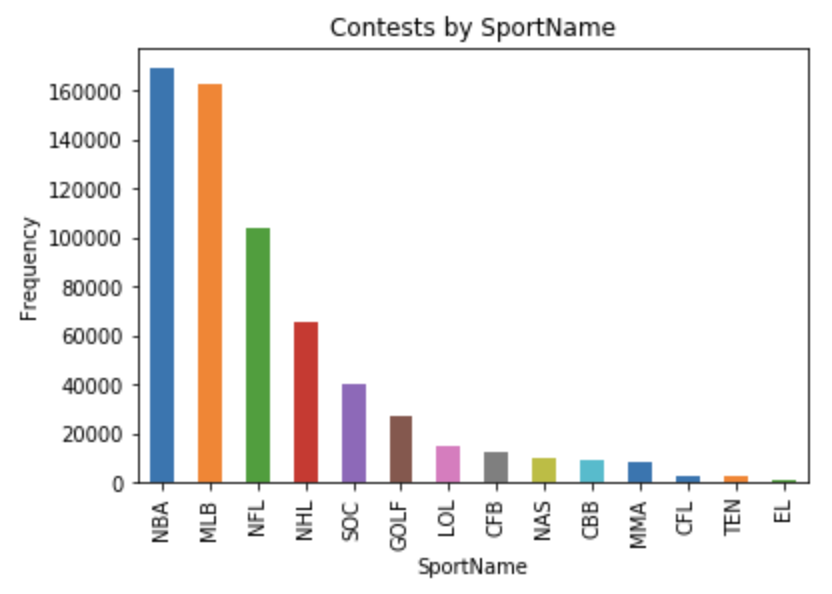
\includegraphics[width=8cm]{body/background/SportName.png}
\caption[SportName Histogram]{A histogram of the number of contests for each SportName sorted in descending order. Approximately 80\% of all contests are of the type NBA, MLB, NFL, or NHL which stand for basketball, baseball, football and hockey respectively.}
\label{fig:sportname}
\end{figure}
%we should describe the codes in the appendix

A typical \textbf{ContestName} might be \textit{CFB 1K Blitz 1,000 Guaranteed}, describing the sport, prizes and occasionally the \textbf{VariantName}, all information coded in other variables. \textbf{EntryFeeAmount} ranges from \$0.10 to \$28,000, but most values fall between one dollar and twenty-seven dollars with a median of five dollars. \textbf{TotalPrizeAmount} ranges from two dollars to 2 million dollars, but most values fall between \$100 and \$25,000, with a median of \$500. Similarly, \textbf{TopPrize} ranges from \$1.80 and 2 million dollars, with most prizes between \$20 and \$400. \textbf{MaxNumberPlayers} ranges from 2 to nearly 2 million with a median value of 98. For most contests, \textbf{MaxEntriesPerUser} is one or two, but occasional contests are nearly uncapped, with up to a billion entries available to each user. \textbf{Entries} varies between 1 and over 1 million, but most contests fall between 23 and 441 entries; \textbf{DistinctUsers} varies similarly from 1 to about half a million, with most falling between 23 and 277 distinct users in a contest.

\begin{figure}
\centering
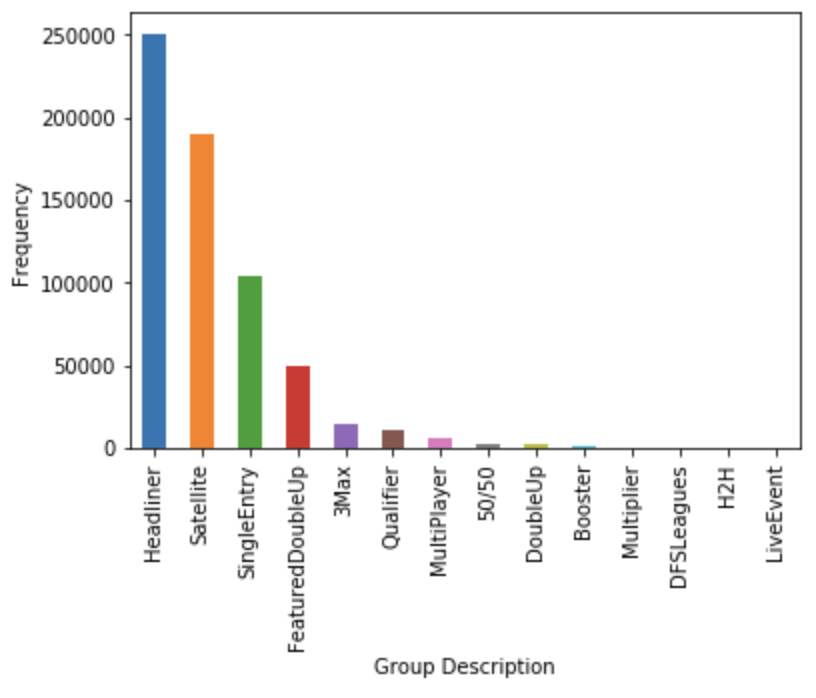
\includegraphics[width=8cm]{body/background/ContestGroup.png}
\caption[ContestGroup Histogram]{A histogram of the number of contests for each ContestGroup sorted in descending order. Approximately 94\% of all contests are of the type Headliner, Satellite, SingleEntry, or FeaturedDoubleUp.}
\label{fig:contestgroup}
\end{figure}
%we should describe the groups in the appendix

Most contests fall into three categories of \textbf{ContestGroup}: Headliner, which are the main featured contests; Satellite, which winning allows users to enter another contest for a large prize pool; and Single Entry, for which only one entry per user is allowed. \textbf{NumGames}, describing how many professional games a contest covers, is less than eight 75\% of the time, but can be as many as 64 in our dataset. The number of players in the draft set for a contest, or \textbf{DraftablePlayersInSet}, has a median of 166, but is skewed left with a mean value of about 316. Finally, the draft groups that DraftKings creates consist of all users who have participated in similar contests in the past, as defined by the company. These groups can be as small as 0 and as large as 750,000, but most fall between 7,000 and 62,000. \newline


\subsection{Time Series Data}

The Time Series Data was separated into monthly files. For example, one file 2015-09.csv contained all the entry information for contests running in September of 2015. Each row in these monthly entry files included the \textbf{ContestId}, minutes until the contest closes and the number of entries the contest received in the last minute. An example best explains this structure. In Table \ref{tab:series}, between 2 minutes to close and 1 minute to close, Contest 7962690 received 18 entries. Likewise from 1 minutes to close to 0 minutes to close, the contest received 24 entries. Unfortunately, many contests began near the end of the month causing some individual contest data to be split between multiple month files. This presented a technical challenge in aggregating data discussed more in the methodology section.

Using the time series data, we can sum the entries in every interval to identify the total number of entries a contest receives at any filled minute prior to the contest start. If the entries found in the series files is equal to the entries in the Header Data, we say the the contest has filled. In the complete dataset, approximately 91.3\% of contests fill. 

\begin{table}
\centering
\begin{tabular}{| c | c | c |}
\hline
\textbf{Contest ID} & \textbf{Minutes Remaining in Contest} & \textbf{Entries in Last Minute}  \\ 
\hline
7962690 & 1000 & 3  \\  
\hline
7962690 & 999 & 4   \\
\hline
7962690 & 997 & 2   \\
\hline
\vdots & \vdots & \vdots \\
\hline
7962690 & 2 & 20   \\
\hline
7962690 & 1 & 18   \\
\hline
7962690 & 0 & 24   \\
\hline
7865930 & 600 & 2  \\  
\hline
7865930 & 596 & 1   \\
\hline
7865930 & 594 & 2   \\
\hline
\vdots & \vdots & \vdots \\
\hline
\end{tabular}
\caption[Raw Time Series Data Example]{This is an example of the form the times series data was originally provided in. Each included columns for unique contest ID, minutes until the contest closed, and the number of entries received in the last minute. Data only appears if users entered the contest within the last minute, so gaps in ``Minutes Remaining in Contest'' can appear if no new entries were made that minute. Additionally, each file contained multiple thousands of unique contests (this fake set shows only two, but would surely have thousands more).}
\label{tab:series}
\end{table}

\subsection{How to Approach the Problem}
Given all this information about the data set, we are still left with the issue of deciding how to best utilize it for the purpose of predicting contest profitability. 

To summarize the points already made, the dataset is known to be large, both in size and dimension, as there are over 600,000 entries each with 21 potential features to analyze. Prediction on data of this scale is commonly performed using flexible modeling techniques that can better accommodate its complexities. One draw-back of flexible modeling, though, is that as the flexibility increases the interpretability of the result decreases. That is to say, it becomes more difficult to discern trends between the explanatory variable(s) and the response variable as flexible increases. In this application, we care more about the actual prediction than being able to interpret trends so it would seem a flexible model may be what we want.

We should also recall that the dataset includes time series data for each contest, which would likely be far too large for any single modeling scheme to incorporate in its entirety. Assuming we aim to utilize some kind of flexible technique, it could be good to try to characterize each contest's time series data by fitting a common function to them. Then, using the predicted function's parameters as new features in addition to the initial 21 header data features, we may be able to achieve a higher level of accuracy from the chosen flexible technique.

Lastly, this dataset seems to contain both categorical and numerical features, so whatever technique we apply will need to be able to handle both at once. Moreover, all the data we have can be easily labeled as ``Success'' or ``Failure''. This means we can directly evaluate the outputs against the known true values. Even better might be if the technique we apply could take advantage of having labeled data to further improve its predictive performance.

With all this in mind, we can conclude that an ideal solution (at least at the theoretical level) would be to use a flexible predictive modeling technique that can handle both numerical and categorical data simultaneously. It would also be preferred if it could utilize labeled data for improved performance and that it use curve fitted functions from the time series data to engineered new features along side the original set. In the realm of data science, one intuitive solution that meets all these requirements is machine learning. 



% There are other key factors that can be learned about the dataset besides the format of each point. Important characteristics of the data set can heavily influence which algorithms will be effective in prediction, such as correlation of features, reliability and data sparsity. Two characteristics of importance in the DraftKings data were sample size and imbalanced data ratio.  

% \subsubsection{Large Sample Size}
% Sample size is an important factor in Machine Learning. Having a larger sample size allows machine learning algorithms to ``learn'' on more data. This leads to greater accuracy when predicting future data points, as algorithms are less likely to overfit on larger sets. A larger sample size also allows for more options when sub sectioning the data. DraftKings' dataset includes 630,466 recorded unique contests from their online website. This is a huge sample size giving us more freedom in algorithm choice. 

% \subsubsection {Imbalanced Data}
% Another note is that the contest results are favored towards filled contest, with about 91 percent of all contests on the platform successfully filling. This is known as imbalanced data. Imbalanced data is a complicated topic, so a deeper dive is need to understand how this affects our predictions. We explore imbalanced data more in Chapter 2.4.

% Key takeaways to understand our data is that the dataset is imbalanced, large, has a large number of features. The goal of our project is detecting contests that will not fill. As a result, we need an algorithm that is consistent, reliable, flexible, and able to analyze a high number of dimensions.


